\chapter{Técnicas de laboratório I: segurança, medição e separação}\label{ch:b1:lab-techniques-1}

Dois estudantes recristalizam o mesmo lote de aspirina e medem seu ponto
de fusão no mesmo banco aquecido. Um lê \qty{134}{\celsius}, o outro
\qty{136}{\celsius}. Eles discordam? O produto é puro? Nenhuma das duas
perguntas pode ser respondida apenas com os dois números: uma medida só
vale algo com sua incerteza, e uma comparação só com uma regra. Este
último capítulo reúne o lado prático do ano: como ler os \omterm{def:b1:lab-techniques-1:hazard}{perigos} do que
está na bancada, como enunciar um valor medido e sua incerteza e
compará-lo com outro, e como as operações clássicas do laboratório de
química orgânica --- extração, filtração, \omterm{def:b1:lab-techniques-1:recrystallisation}{recristalização}, destilação ---
separam um produto do que o cerca e depois verificam que ele é puro.

\begin{recall}
A \omterm{def:b1:precipitation:solubility}{solubilidade} e a miscibilidade a partir das forças intermoleculares,
os \omterm{def:b1:intermolecular-forces-solvents:solvent-classes}{solventes polares} e apolares (\cref{ch:b1:intermolecular-forces-solvents});
buretas, pipetas e o \omterm{def:b1:titration-methods:titration}{ponto final} de uma \omterm{def:b1:titration-methods:titration}{titulação} (\cref{ch:b1:titration-methods}).
O Livro 1 (ano 10) apresentou a extração líquido--líquido, a
\omterm{def:b1:lab-techniques-1:recrystallisation}{recristalização}, a cromatografia em camada delgada e o \omterm{def:b1:extent-q-and-k:fractional-extent}{rendimento} de uma
síntese; aqui eles ganham seus números.
\end{recall}

\begin{omfigure}
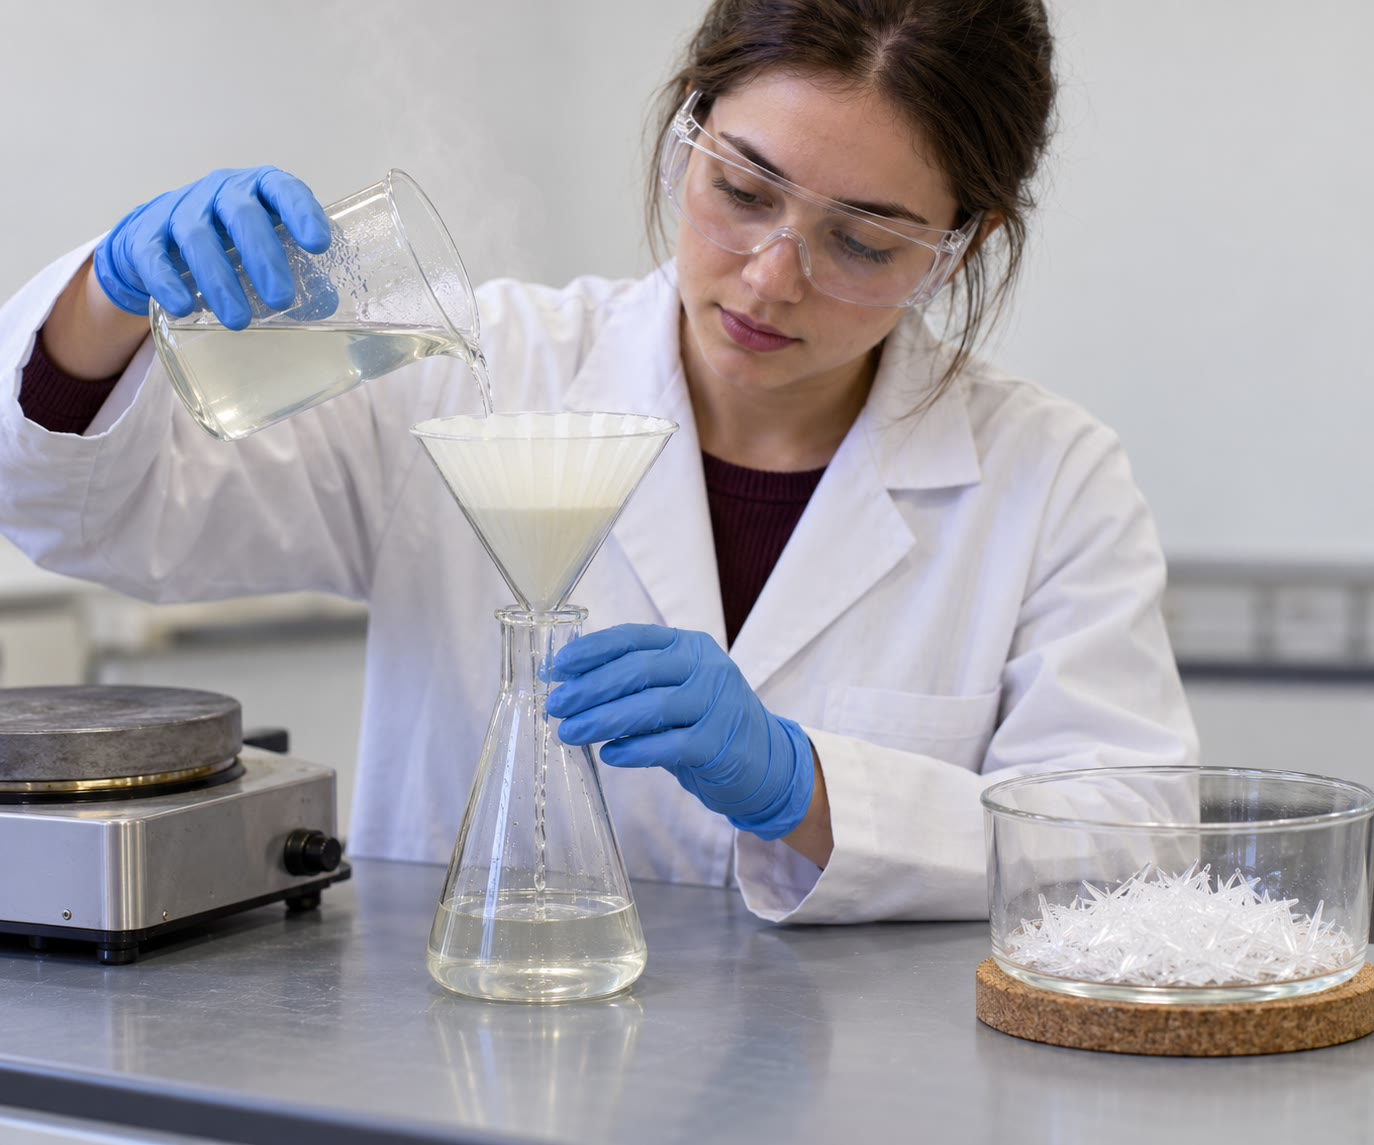
\includegraphics[width=0.5\linewidth]{images/book2/ai/b1-29-recrystallisation.jpg}

{\small Filtração a quente durante uma \omterm{def:b1:lab-techniques-1:recrystallisation}{recristalização}: óculos, luvas e
jaleco; a solução quente passa por um papel de filtro pregueado, que retém
as impurezas insolúveis. Agulhas de um produto recristalizado esperam no
recipiente à direita.}
\end{omfigure}

\section{Os perigos e seus rótulos}

\begin{definition}[Perigo e risco]\label{def:b1:lab-techniques-1:hazard}
Um \emph{perigo}\index{perigo} é a propriedade intrínseca de uma substância
(ou de uma situação) que pode causar dano: inflamabilidade, corrosividade,
toxicidade. O \emph{risco}\index{risco} é a probabilidade de que o dano
ocorra de fato, e sua gravidade, nas condições de uso dadas: ele depende
do perigo e da exposição (quantidade, concentração, duração, via,
proteção).
\end{definition}

Um \omterm{def:b1:lab-techniques-1:hazard}{perigo} não pode ser mudado sem mudar a substância; um \omterm{def:b1:lab-techniques-1:hazard}{risco} é reduzido
agindo sobre a exposição: uma quantidade menor, uma solução mais diluída,
uma capela, luvas e óculos, ou um reagente menos perigoso para o mesmo
trabalho.

\begin{definition}[Rotulagem GHS]\label{def:b1:lab-techniques-1:ghs}
Os rótulos dos produtos químicos seguem o Sistema Globalmente Harmonizado (GHS).
\begin{itemize}
  \item Um \emph{pictograma de perigo}\index{pictograma de perigo} é um
        símbolo preto sobre um losango branco de borda vermelha; há nove,
        de \texttt{GHS01} a \texttt{GHS09}.
  \item A \emph{palavra de advertência}\index{palavra de advertencia@palavra de advertência} é \emph{Perigo} para
        as categorias de \omterm{def:b1:lab-techniques-1:hazard}{perigo} mais graves e \emph{Atenção} para as menos
        graves; um rótulo traz só uma, a mais grave.
  \item Uma \emph{frase de perigo}\index{frase de perigo} é uma frase
        padronizada, codificada por H seguido de três algarismos, que
        descreve um \omterm{def:b1:lab-techniques-1:hazard}{perigo}: H2xx \omterm{def:b1:lab-techniques-1:hazard}{perigos} físicos, H3xx \omterm{def:b1:lab-techniques-1:hazard}{perigos} para a
        saúde, H4xx \omterm{def:b1:lab-techniques-1:hazard}{perigos} para o meio ambiente.
  \item Uma \emph{frase de precaução}\index{frase de precaucao@frase de precaução},
        codificada por P e três algarismos, indica uma medida a tomar: P1xx
        gerais, P2xx prevenção, P3xx resposta, P4xx armazenamento, P5xx
        descarte.
  \item A \emph{ficha de dados de segurança}\index{ficha de dados de seguranca@ficha de dados de segurança} é
        o documento que o fornecedor entrega com um produto, em seções
        padronizadas: identificação, \omterm{def:b1:lab-techniques-1:hazard}{perigos}, composição, primeiros
        socorros, combate a incêndio, manuseio e armazenamento, controle
        de exposição e proteção, propriedades físicas e químicas,
        estabilidade, toxicidade, descarte e transporte.
\end{itemize}
\end{definition}

\begin{omfigure}
\setlength{\tabcolsep}{5pt}
\begin{tabular}{ccccc}
\begin{tabular}[t]{@{}c@{}}\ghs[1.25cm]{GHS01}\\[2pt]\footnotesize GHS01\\\footnotesize explosivo\end{tabular} &
\begin{tabular}[t]{@{}c@{}}\ghs[1.25cm]{GHS02}\\[2pt]\footnotesize GHS02\\\footnotesize inflamável\end{tabular} &
\begin{tabular}[t]{@{}c@{}}\ghs[1.25cm]{GHS03}\\[2pt]\footnotesize GHS03\\\footnotesize oxidante\end{tabular} &
\begin{tabular}[t]{@{}c@{}}\ghs[1.25cm]{GHS04}\\[2pt]\footnotesize GHS04\\\footnotesize gás sob pressão\end{tabular} &
\begin{tabular}[t]{@{}c@{}}\ghs[1.25cm]{GHS05}\\[2pt]\footnotesize GHS05\\\footnotesize corrosivo\end{tabular} \\[8pt]
\begin{tabular}[t]{@{}c@{}}\ghs[1.25cm]{GHS06}\\[2pt]\footnotesize GHS06\\\footnotesize toxicidade aguda\end{tabular} &
\begin{tabular}[t]{@{}c@{}}\ghs[1.25cm]{GHS07}\\[2pt]\footnotesize GHS07\\\footnotesize nocivo, irritante\end{tabular} &
\begin{tabular}[t]{@{}c@{}}\ghs[1.25cm]{GHS08}\\[2pt]\footnotesize GHS08\\\footnotesize perigo à saúde\end{tabular} &
\begin{tabular}[t]{@{}c@{}}\ghs[1.25cm]{GHS09}\\[2pt]\footnotesize GHS09\\\footnotesize meio ambiente\end{tabular} & \\
\end{tabular}

\smallskip
{\small Os nove pictogramas GHS: bomba explodindo, chama, chama sobre um
círculo, cilindro de gás, corrosão, caveira com ossos cruzados, ponto de
exclamação, perigo à saúde (efeitos de longo prazo: câncer, mutações,
reprodução, sensibilização das vias respiratórias, aspiração) e meio ambiente.}
% ledger: ghspic:GHS01, ghspic:GHS02, ghspic:GHS03, ghspic:GHS04,
% ghspic:GHS05, ghspic:GHS06, ghspic:GHS07, ghspic:GHS08, ghspic:GHS09
\end{omfigure}

\begin{example}[Ler o rótulo do etanol]
Um frasco de etanol traz os pictogramas GHS02 e GHS07, a \omterm{def:b1:lab-techniques-1:ghs}{palavra de
advertência} \emph{Perigo} e as frases H225 (líquido e vapores altamente
inflamáveis, um \omterm{def:b1:lab-techniques-1:hazard}{perigo} físico, cuja categoria exige \emph{Perigo}) e H319
(provoca irritação ocular grave, um \omterm{def:b1:lab-techniques-1:hazard}{perigo} para a saúde, \emph{Atenção}
por si só). Suas \omterm{def:b1:lab-techniques-1:ghs}{frases de precaução} incluem P210 (mantenha afastado do
calor, de faíscas e de chamas abertas; não fume), P233 (mantenha o
recipiente hermeticamente fechado), P280 (use luvas e proteção ocular),
P305+P351+P338 (em caso de contato com os olhos: enxágue cuidadosamente
com água durante vários minutos, remova as lentes de contato, continue
enxaguando) e P403+P235 (armazene em local bem ventilado, mantenha em
local fresco). As consequências práticas: nenhuma chama na bancada onde
se usa etanol, óculos, um frasco fechado.
\end{example}
% ledger: ghs:ethanol, hstat:H225, hstat:H319, pstat:P210, pstat:P233,
% pstat:P280, pstat:P305+P351+P338, pstat:P403+P235

\begin{method}[Preparar uma aula prática a partir das fichas de dados de segurança]\label{met:b1:lab-techniques-1:read-sds}
Para cada substância usada ou formada:
\begin{enumerate}
  \item leia seus pictogramas, sua \omterm{def:b1:lab-techniques-1:ghs}{palavra de advertência} e suas frases H
        (seção 2 da ficha), e anote os \omterm{def:b1:lab-techniques-1:hazard}{perigos} físicos (fogo, pressão,
        reatividade) separadamente dos \omterm{def:b1:lab-techniques-1:hazard}{perigos} para a saúde e o meio ambiente;
  \item para cada operação (pesagem, aquecimento, transferência,
        filtração), estime a exposição: quantidade, estado (um líquido
        volátil ou um pó fino chega aos pulmões), duração;
  \item escolha as medidas: substituição por um reagente menos perigoso,
        escala menor, capela, depois proteção individual (frases P2xx);
  \item planeje a resposta a um incidente (P3xx: olhos, pele, ingestão,
        fogo) e o destino de cada resíduo (P5xx).
\end{enumerate}
\end{method}

\begin{inthelab}[Resíduos]
Por padrão, nada vai para a pia. Os solventes orgânicos são recolhidos em
dois recipientes, halogenados (diclorometano, clorofórmio) e não
halogenados (etanol, propanona, ciclo-hexano, etanoato de etila), pois são
tratados de modo diferente; as soluções aquosas ácidas e básicas são
neutralizadas antes do descarte; as soluções de íons de metais pesados
(cromo, cobre, prata) têm seus próprios recipientes; o vidro quebrado e os
sólidos contaminados são mantidos separados do lixo comum. A frase P273,
``evite a liberação para o meio ambiente'', em um rótulo lembra que o
recipiente de resíduos, e não o ralo, é o fim do experimento.
% ledger: pstat:P273
\end{inthelab}

\section{Medição e incerteza}

Um valor medido nunca é o valor exato da grandeza medida: repita a medição
e o resultado muda um pouco; leia a escala e o último algarismo é uma
estimativa. A incerteza diz a que distância do valor medido o valor
verdadeiro pode razoavelmente estar.

\begin{definition}[Incerteza de medição]\label{def:b1:lab-techniques-1:uncertainty}
\begin{itemize}
  \item A \emph{incerteza de medição}\index{incerteza de medicao@incerteza de medição}
        é um parâmetro que caracteriza a dispersão dos valores que podem
        razoavelmente ser atribuídos à grandeza medida.
  \item A \emph{incerteza-padrão}\index{incerteza-padrao@incerteza-padrão} $u(x)$
        é essa incerteza expressa como um desvio-padrão.
  \item Uma \emph{avaliação do tipo A}\index{avaliacao do tipo A@avaliação do tipo A} obtém $u$
        pela análise estatística de uma série de medições repetidas; uma
        \emph{avaliação do tipo B}\index{avaliacao do tipo B@avaliação do tipo B} a obtém por
        qualquer outro meio: a graduação de um instrumento, a tolerância
        declarada pelo fabricante, um certificado de calibração, o número
        de algarismos de um valor tabelado.
  \item A \emph{incerteza expandida}\index{incerteza expandida}
        $U = k\,u$ é a incerteza-padrão multiplicada por um fator de
        abrangência $k$, em geral $k = 2$; para uma distribuição normal, o
        intervalo $x \pm 2u$ contém o valor verdadeiro com uma probabilidade
        de cerca de \qty{95}{\percent}.
  \item A \emph{incerteza relativa}\index{incerteza relativa} é
        $u(x)/|x|$, muitas vezes dada em porcentagem.
\end{itemize}
\end{definition}

\begin{proposition}[Avaliação do tipo A]\label{prop:b1:lab-techniques-1:type-a}
Se são feitas $n$ medições independentes $x_1, \dots, x_n$ da mesma
grandeza, a melhor estimativa é sua média $\bar x$; o desvio-padrão
experimental é
\[
  s = \sqrt{\frac{1}{n-1} \sum_{i=1}^{n} (x_i - \bar x)^2},
\]
e a \omterm{def:b1:lab-techniques-1:uncertainty}{incerteza-padrão} da média é $u(\bar x) = s/\sqrt{n}$.
\end{proposition}
\begin{proof}[\omnameProof]
\emph{Admitido neste nível}; a estatística das medições repetidas,
incluindo o coeficiente de Student usado quando $n$ é pequeno, é tratada
no volume do 2.º~ano.
\end{proof}

\begin{omfigure}
\begin{tikzpicture}
\begin{axis}[width=7.4cm, height=5cm, xlabel={volume no ponto final (\unit{mL})},
  ylabel={número de leituras}, ymin=0, ymax=8.5, xmin=12.2, xmax=12.7,
  xtick={12.2,12.3,12.4,12.5,12.6,12.7},
  xticklabel style={/pgf/number format/fixed, /pgf/number format/precision=1},
  axis lines=left, every axis plot/.append style={line join=round}]
  \addplot[ybar, bar width=0.045, fill=omDef!35, draw=omDef!80!black]
    table[x=V, y=count] {figdata/out/bachelor-1-type-a-uncertainty-a.dat};
  \addplot[omThm, thick, smooth]
    table[x=V, y=g] {figdata/out/bachelor-1-type-a-uncertainty-b.dat};
  \draw[omProp, thick, <->] (axis cs:12.384,7.6) -- (axis cs:12.526,7.6);
  \node[omProp, font=\small, above] at (axis cs:12.455,7.6) {$\bar V \pm s$};
\end{axis}
\end{tikzpicture}\hspace{0.6cm}%
\begin{tikzpicture}
\begin{axis}[width=5.6cm, height=5cm, xlabel={$x - x_0$}, ylabel={densidade},
  ymin=0, ymax=0.8, xmin=-1.6, xmax=1.6, xtick={-1,0,1},
  xticklabels={$-a$, $0$, $a$}, ytick={0.5}, yticklabels={$\frac{1}{2a}$},
  axis lines=left]
  \addplot[omDef!80!black, thick, fill=omDef!25] coordinates
    {(-1,0) (-1,0.5) (1,0.5) (1,0)} \closedcycle;
  \draw[omProp, thick, <->] (axis cs:-0.577,0.62) -- (axis cs:0.577,0.62);
  \node[omProp, font=\small, above] at (axis cs:0,0.62) {$\pm a/\sqrt3$};
\end{axis}
\end{tikzpicture}

{\small À esquerda: vinte leituras do mesmo \omterm{def:b1:titration-methods:titration}{ponto final} de \omterm{def:b1:titration-methods:titration}{titulação}
(dados ilustrativos), lidas a \qty{0.05}{mL}, com a curva normal de mesma
média $\bar V = \qty{12.455}{mL}$ e mesmo desvio-padrão $s = \qty{0.071}{mL}$.
À direita: a distribuição retangular de uma \omterm{def:b1:lab-techniques-1:uncertainty}{avaliação do tipo B}, um valor
que só se sabe estar entre $x_0 - a$ e $x_0 + a$; seu desvio-padrão é
$a/\sqrt3$.}
\end{omfigure}

\begin{example}[Vinte pontos finais]
Para as vinte leituras da figura, $\bar V = \qty{12.455}{mL}$,
$s = \qty{0.071}{mL}$ e $u(\bar V) = 0.071/\sqrt{20} = \qty{0.016}{mL}$.
Uma leitura é incerta em cerca de $s$; a média de vinte, em cerca de
$s/\sqrt{20}$, quatro vezes e meia menos. O resultado é
$V = \qty{12.46}{mL}$ com $U = 2u = \qty{0.03}{mL}$.
\end{example}

\begin{proposition}[Avaliação do tipo B para uma distribuição retangular]\label{prop:b1:lab-techniques-1:type-b}
Se tudo o que se sabe de uma grandeza é que ela está, com igual
probabilidade, em qualquer ponto entre $x_0 - a$ e $x_0 + a$, sua
\omterm{def:b1:lab-techniques-1:uncertainty}{incerteza-padrão} é
\[
  u = \frac{a}{\sqrt3}.
\]
\end{proposition}
\begin{proof}
A densidade de probabilidade é $1/(2a)$ em $[x_0 - a, x_0 + a]$ e zero
fora dele; sua média é $x_0$ por simetria e sua variância é
\[
  u^2 = \int_{x_0-a}^{x_0+a} (x - x_0)^2 \frac{\mathrm{d}x}{2a}
      = \frac{1}{2a} \left[\frac{t^3}{3}\right]_{-a}^{a}
      = \frac{1}{2a}\cdot\frac{2a^3}{3} = \frac{a^2}{3}. \qedhere
\]
\end{proof}

\begin{example}[Uma leitura e uma tolerância]
Uma bureta graduada a cada \qty{0.1}{mL} é lida a meia divisão: a leitura
fica a $\pm\qty{0.05}{mL}$ do valor anotado, de modo que
$u = 0.05/\sqrt3 = \qty{0.029}{mL}$. Uma pipeta de \qty{20}{mL} cujo
fabricante declara uma tolerância de $\pm\qty{0.03}{mL}$ fornece seu volume com
$u = 0.03/\sqrt3 = \qty{0.017}{mL}$. Um valor tabelado dado como
\qty{135}{\celsius} é conhecido a $\pm\qty{0.5}{\celsius}$: $u = \qty{0.29}{\celsius}$.
\end{example}

\begin{proposition}[Combinar incertezas]\label{prop:b1:lab-techniques-1:combine}
Para grandezas independentes: se $y = x_1 + x_2$ ou $y = x_1 - x_2$, então
$u(y)^2 = u(x_1)^2 + u(x_2)^2$; se $y = x_1 x_2$ ou $y = x_1/x_2$, então
\[
  \left(\frac{u(y)}{y}\right)^2 = \left(\frac{u(x_1)}{x_1}\right)^2
  + \left(\frac{u(x_2)}{x_2}\right)^2 .
\]
Várias fontes de incerteza sobre a mesma grandeza (uma parte do tipo A e
partes do tipo B) se combinam da mesma maneira, como uma soma de quadrados.
\end{proposition}
\admitted

São os quadrados, e não as próprias incertezas, que se somam: dois erros
independentes raramente empurram no mesmo sentido com toda a intensidade.
Um volume titulado é a diferença de duas leituras da bureta, de modo que
sua incerteza de leitura é
$\sqrt2 \times \qty{0.029}{mL} = \qty{0.041}{mL}$; e uma fonte grande de
incerteza domina as outras, e é ali que se deve buscar uma melhora. A
regra geral, com derivadas parciais, pertence ao volume do 2.º~ano.

\begin{method}[Expressar um resultado]\label{met:b1:lab-techniques-1:report-result}
\begin{enumerate}
  \item Liste as fontes de incerteza; avalie cada uma como \omterm{def:b1:lab-techniques-1:uncertainty}{incerteza-padrão}
        (tipo A a partir de uma série, tipo B como $a/\sqrt3$ a partir de
        uma semiamplitude).
  \item Combine-as como uma soma de quadrados (\cref{prop:b1:lab-techniques-1:combine}).
  \item Dê a \omterm{def:b1:lab-techniques-1:uncertainty}{incerteza expandida} $U = 2u$ com um ou dois algarismos
        significativos, e arredonde o valor na mesma casa decimal:
        $x = (\text{valor} \pm U)$ unidade, $k = 2$.
\end{enumerate}
\end{method}

\begin{definition}[Desvio normalizado]\label{def:b1:lab-techniques-1:z-score}
O \emph{desvio normalizado}\index{desvio normalizado} (ou escore $z$)
entre dois valores independentes $x_1$ e $x_2$ da mesma grandeza, de
incertezas-padrão $u_1$ e $u_2$, é
\[
  z = \frac{|x_1 - x_2|}{\sqrt{u_1^2 + u_2^2}} .
\]
Os dois valores são ditos compatíveis quando $z \le 2$; um valor medido é
compatível com um valor de referência sob a mesma condição.
\end{definition}

\begin{example}[Os dois estudantes]
Os dois pontos de fusão da abertura, \qty{134}{\celsius} e
\qty{136}{\celsius}, foram obtidos cada um com uma \omterm{def:b1:lab-techniques-1:uncertainty}{incerteza-padrão} de
\qty{0.8}{\celsius} (leitura e calibração do banco). Então
$z = 2/\sqrt{0.8^2 + 0.8^2} = 1.8 \le 2$: os estudantes concordam. Sua
média, \qty{135}{\celsius}, também é compatível com o ponto de fusão
tabelado da aspirina, \qty{135}{\celsius} sob aquecimento rápido. Um valor
tabelado dado na unidade tem $u = 0.5/\sqrt3 = \qty{0.29}{\celsius}$, de
modo que uma única leitura com $u = \qty{0.8}{\celsius}$ é compatível com
ele enquanto estiver a menos de $2\sqrt{0.8^2 + 0.29^2} = \qty{1.7}{\celsius}$
dele: uma leitura abaixo de cerca de \qty{133}{\celsius} teria indicado um
produto impuro.
\end{example}
% ledger: mp:aspirin

\section{Separar}

\begin{definition}[Coeficiente de partição]\label{def:b1:lab-techniques-1:partition-coefficient}
Quando um soluto A se reparte, no equilíbrio, entre dois solventes
imiscíveis, uma \omterm{def:b1:extent-q-and-k:system}{fase} orgânica e uma \omterm{def:b1:extent-q-and-k:system}{fase} aquosa, a razão entre suas
concentrações
\[
  K = \frac{[\mathrm{A}]_{\mathrm{org}}}{[\mathrm{A}]_{\mathrm{aq}}}
\]
é, para soluções diluídas a uma dada temperatura, uma constante: o
\emph{coeficiente de partição}\index{coeficiente de particao@coeficiente de partição} de A entre os
dois solventes.
\end{definition}

\begin{proposition}[Várias extrações valem mais que uma]\label{prop:b1:lab-techniques-1:multiple-extractions}
Um volume $V_a$ de solução aquosa é extraído $n$ vezes, a cada vez com um
volume novo $V_o$ de solvente orgânico. A fração de A que resta na \omterm{def:b1:extent-q-and-k:system}{fase}
aquosa é
\[
  f_n = \left(1 + K \frac{V_o}{V_a}\right)^{-n}.
\]
Para um volume total de solvente fixo, $n$ porções pequenas extraem mais
que uma porção grande.
\end{proposition}
\begin{proof}
Seja $m$ a quantidade de A na \omterm{def:b1:extent-q-and-k:system}{fase} aquosa antes de uma extração, e $m'$
depois. No equilíbrio, a \omterm{def:b1:extent-q-and-k:system}{fase} orgânica contém $m - m'$, e
$K = \dfrac{(m - m')/V_o}{m'/V_a}$, logo $m - m' = K\dfrac{V_o}{V_a} m'$ e
$m' = m\big/\bigl(1 + K V_o/V_a\bigr)$. Cada extração multiplica a
quantidade restante pelo mesmo fator; depois de $n$ delas, $f_n$ é a
$n$-ésima potência. Com um volume total $V$ dividido em $n$ porções $V/n$,
$\ln f_n = -n \ln(1 + KV/(nV_a))$; como $\ln(1+t)/t$ decresce com $t$,
$n \ln(1 + t/n)$ cresce com $n$ para $t = KV/V_a > 0$, e $f_n$
decresce, tendendo ao limite $\mathrm{e}^{-KV/V_a}$.
\end{proof}

\begin{example}[Uma porção ou três]
Um soluto com $K = 4$ é extraído de \qty{100}{mL} de água com
\qty{60}{mL} de etanoato de etila. Em uma porção,
$f_1 = 1/(1 + 4 \times 0.6) = 0.29$: \qty{71}{\percent} são extraídos. Em
três porções de \qty{20}{mL}, $f_3 = (1 + 4 \times 0.2)^{-3} = 0.17$:
\qty{83}{\percent}. O etanoato de etila ($\rho = \qty{0.90}{g/cm^3}$) é a
camada superior no funil de separação; o diclorometano
($\rho = \qty{1.33}{g/cm^3}$) seria a inferior.
\end{example}
% ledger: rho:ethyl-acetate, rho:CH2Cl2, rho:water

A filtração separa um sólido de um líquido. Por gravidade, através de um
papel pregueado em um funil, ela retém uma impureza insolúvel de uma
solução quente que não deve esfriar no caminho (filtração a quente, como
na fotografia do início do capítulo). Sob pressão reduzida, em um funil de
Büchner sobre um kitassato (como desenhado no Livro 1), ela recolhe um
sólido rapidamente e o deixa quase seco; o sólido é lavado no filtro com
um pouco de solvente frio.

\begin{definition}[Recristalização]\label{def:b1:lab-techniques-1:recrystallisation}
A \emph{recristalização}\index{recristalizacao@recristalização} purifica um sólido
dissolvendo-o no mínimo de um solvente quente em que ele é muito solúvel
a quente e pouco solúvel a frio, e deixando-o depois cristalizar no
resfriamento; as impurezas ou ficam dissolvidas no solvente frio (a
água-mãe) ou, sendo insolúveis, são removidas antes por filtração a quente.
\end{definition}

\begin{method}[Recristalizar um sólido]\label{met:b1:lab-techniques-1:recrystallise}
\begin{enumerate}
  \item Escolha o solvente: o produto muito solúvel a quente e pouco
        solúvel a frio, as impurezas solúveis mesmo a frio, nenhuma
        reação com o produto, uma temperatura de ebulição abaixo do ponto
        de fusão do produto; uma mistura de dois solventes \omterm{def:b1:intermolecular-forces-solvents:miscibility}{miscíveis}
        (etanol e água) pode ser ajustada ao produto.
  \item Dissolva o sólido bruto no mínimo de solvente em ebulição,
        adicionado em pequenas porções, sob refluxo se o solvente for
        volátil ou inflamável.
  \item Se restar uma impureza insolúvel, filtre a quente.
  \item Deixe a solução esfriar lentamente, depois em gelo: um
        resfriamento lento dá \omterm{def:b1:crystals-metals:crystal}{cristais} maiores e mais puros, que aprisionam
        menos água-mãe.
  \item Filtre sob pressão reduzida, lave com um pouco de solvente
        gelado, seque, pese; verifique a pureza (ponto de fusão, CCD).
\end{enumerate}
\end{method}

\begin{example}[O preço da pureza]
A aspirina se dissolve em água a cerca de \qty{3.3}{g/L} a \qty{25}{\celsius}
e \qty{10}{g/L} a \qty{37}{\celsius}, muito mais perto da temperatura de
ebulição. Se \qty{40}{mL} de água-mãe e \qty{10}{mL} de água de lavagem
saem do filtro a \qty{25}{\celsius}, eles levam cerca de
$\qty{0.050}{L} \times \qty{3.3}{g/L} = \qty{0.17}{g}$ de aspirina, qualquer
que seja sua pureza. Cada mililitro de solvente além do mínimo custa
\omterm{def:b1:extent-q-and-k:fractional-extent}{rendimento}.
\end{example}
% ledger: sol:aspirin-25, sol:aspirin-37

Um líquido é purificado, ou dois líquidos de temperaturas de ebulição bem
separadas são separados, por \emph{destilação simples}: a mistura é
fervida, o vapor, mais rico no componente mais volátil, é condensado e
recolhido. A temperatura no braço lateral é a do vapor que destila;
enquanto ela permanece constante, uma substância pura está passando.
Líquidos de temperaturas de ebulição próximas exigem a destilação
fracionada, com uma coluna entre o balão e a cabeça, tratada com os
diagramas líquido--vapor do volume do 2.º~ano.

\begin{omfigure}
\begin{tikzpicture}[font=\small, scale=0.95]
  \pic[transform shape] at (0,0) {heatingmantle};
  \pic[transform shape] at (0,0) {rbflask={0.45}{orange!25}};
  \foreach \x/\y in {-0.35/0.25,0.05/0.18,0.35/0.3}
    \fill[black!55] (\x,\y) circle (0.06);
  \pic[transform shape] (s) at (0,3.0) {stillhead};
  \pic[transform shape] at ($(s-top)+(0,-0.75)$) {thermometer};
  \pic[transform shape, rotate=-20] (c) at (s-arm) {liebig={3.4}};
  \coordinate (cend) at ($(s-arm)+(-20:3.4)$);
  \pic[transform shape] (a) at (cend) {adapter};
  \pic[transform shape] at ($(a-tip)+(0,-2.4)$) {erlenmeyer={0.22}{orange!12}};
  \draw[<-, omProp, thick] (0.12,3.72) -- (-1.4,4.4) node[left, text=black,
    align=right] {bulbo do termômetro\\ no nível do braço lateral};
  \draw[<-, omProp, thick] ($(s-arm)+(-20:0.65)+(0.65,0.65)$) -- ++(0.2,0.9)
    node[above, text=black] {saída de água};
  \draw[<-, omProp, thick] ($(s-arm)+(-20:2.7)+(-0.2,-0.6)$) -- ++(0.05,-0.9)
    node[below, text=black] {\shortstack{entrada\\de água}};
  \draw[<-, omProp, thick] (-0.3,0.27) -- (-2.2,0.7) node[left, text=black]
    {pedras de ebulição};
  \draw[<-, omProp, thick] (1.35,-0.6) -- (2.3,-1.1) node[right, text=black]
    {\shortstack[l]{\footnotesize manta\\\footnotesize aquecedora}};
  \draw[<-, omProp, thick] ($(a-tip)+(0.75,-2.0)$) -- ++(1.0,0.2)
    node[right, text=black] {destilado};
\end{tikzpicture}

{\small Destilação simples. O termômetro lê a temperatura do vapor que
entra no condensador; a água de resfriamento entra pela extremidade
inferior do condensador para que a camisa fique cheia; as pedras de
ebulição evitam a ebulição violenta; o aparelho fica aberto ao ar no
recipiente coletor.}
\end{omfigure}

\begin{safety}{\ghs[5mm]{GHS02}}
Um aparelho de destilação nunca é fechado: aquecido, um sistema vedado
explode. As pedras de ebulição são adicionadas ao líquido frio, nunca a
um líquido já quente (ele pode transbordar de imediato). Um destilado
inflamável é recolhido longe de qualquer chama, com o coletor em gelo se
necessário.
\end{safety}

\section{Identificar e verificar a pureza}

\begin{definition}[Fator de retenção]\label{def:b1:lab-techniques-1:retention-factor}
Na cromatografia em camada delgada (CCD), uma mancha da amostra é
depositada sobre uma linha de base perto do pé de uma placa recoberta por
uma \omterm{def:b1:extent-q-and-k:system}{fase} estacionária (sílica); a placa fica em uma cuba fechada com um
pouco de eluente, que sobe pela camada por capilaridade e arrasta as
espécies com velocidades diferentes. O \emph{fator de retenção}\index{fator de retencao@fator de retenção} de uma
espécie é
\[
  R_f = \frac{\text{distância percorrida pela mancha}}
             {\text{distância percorrida pela frente do eluente}},
\]
ambas medidas a partir da linha de base; $0 \le R_f \le 1$, e, para \omterm{def:b1:extent-q-and-k:system}{fase}
estacionária, eluente e temperatura dados, ele caracteriza a espécie.
\end{definition}

Na sílica, que é polar, uma espécie polar é mais retida que uma menos
polar e tem o menor $R_f$; um eluente mais polar faz todas as manchas
subirem mais. Duas espécies com o mesmo $R_f$ em uma placa ainda podem
ser diferentes; dois $R_f$ diferentes provam que elas diferem. Um produto
puro dá uma única mancha.

\begin{omfigure}
\begin{tikzpicture}[font=\small, scale=1.7]
  \pic[transform shape] at (0,0) {tlcplate};
  \draw[omDef!80!black, densely dashed, line width=0.5pt] (-0.7,2.7) -- (0.7,2.7);
  \foreach \x in {-0.4,0,0.4} \fill[black!60] (\x,0.4) circle (0.025);
  \fill[omThm!70] (-0.4,{0.4+0.30*2.3}) ellipse (0.09 and 0.06);
  \fill[omDef!70] (0,{0.4+0.65*2.3}) ellipse (0.09 and 0.06);
  \fill[omThm!70] (0.4,{0.4+0.30*2.3}) ellipse (0.09 and 0.06);
  \fill[omDef!70] (0.4,{0.4+0.65*2.3}) ellipse (0.09 and 0.06);
  \node[below] at (-0.4,0) {A}; \node[below] at (0,0) {B};
  \node[below] at (0.4,0) {M};
  \draw[omProp, thick, |<->|] (0.95,0.4) -- (0.95,{0.4+0.65*2.3})
    node[midway, right] {$d_{\mathrm{B}}$};
  \draw[omProp, thick, |<->|] (1.55,0.4) -- (1.55,2.7)
    node[midway, right] {$d_{\mathrm{frente}}$};
  \draw[omProp, thick, |<->|] (-0.95,0.4) -- (-0.95,{0.4+0.30*2.3})
    node[midway, left] {$d_{\mathrm{A}}$};
  \node[right, align=left, font=\footnotesize] at (0.75,2.85) {frente do eluente};
  \draw[omProp, thick, <-] (-0.6,0.4) -- (-1.2,0.05) node[left, text=black, font=\footnotesize] {linha de base};
\end{tikzpicture}

{\small Uma placa de CCD revelada: as referências A e B e uma mistura M,
depositadas na linha de base. $R_f(\mathrm{A}) = d_{\mathrm{A}}/d_{\mathrm{frente}}
= 0.30$, $R_f(\mathrm{B}) = 0.65$; a mistura mostra as duas manchas, nas
mesmas alturas.}
\end{omfigure}

\begin{method}[Fazer uma CCD]\label{met:b1:lab-techniques-1:tlc}
\begin{enumerate}
  \item Trace a linha de base a lápis a cerca de \qty{1}{cm} do pé; deposite
        pequenas manchas de soluções diluídas da amostra e das referências
        lado a lado.
  \item Ponha alguns milímetros de eluente na cuba (abaixo da linha de
        base), feche-a, deixe a atmosfera saturar; coloque a placa nela.
  \item Retire a placa quando a frente estiver a cerca de \qty{1}{cm} do
        topo; marque a frente imediatamente; seque.
  \item Revele as manchas incolores (lâmpada ultravioleta sobre uma placa
        fluorescente, vapor de iodo, um corante); circule-as a lápis.
  \item Meça as distâncias a partir da linha de base e calcule cada $R_f$;
        compare a amostra com as referências na mesma placa.
\end{enumerate}
\end{method}

\begin{omfigure}
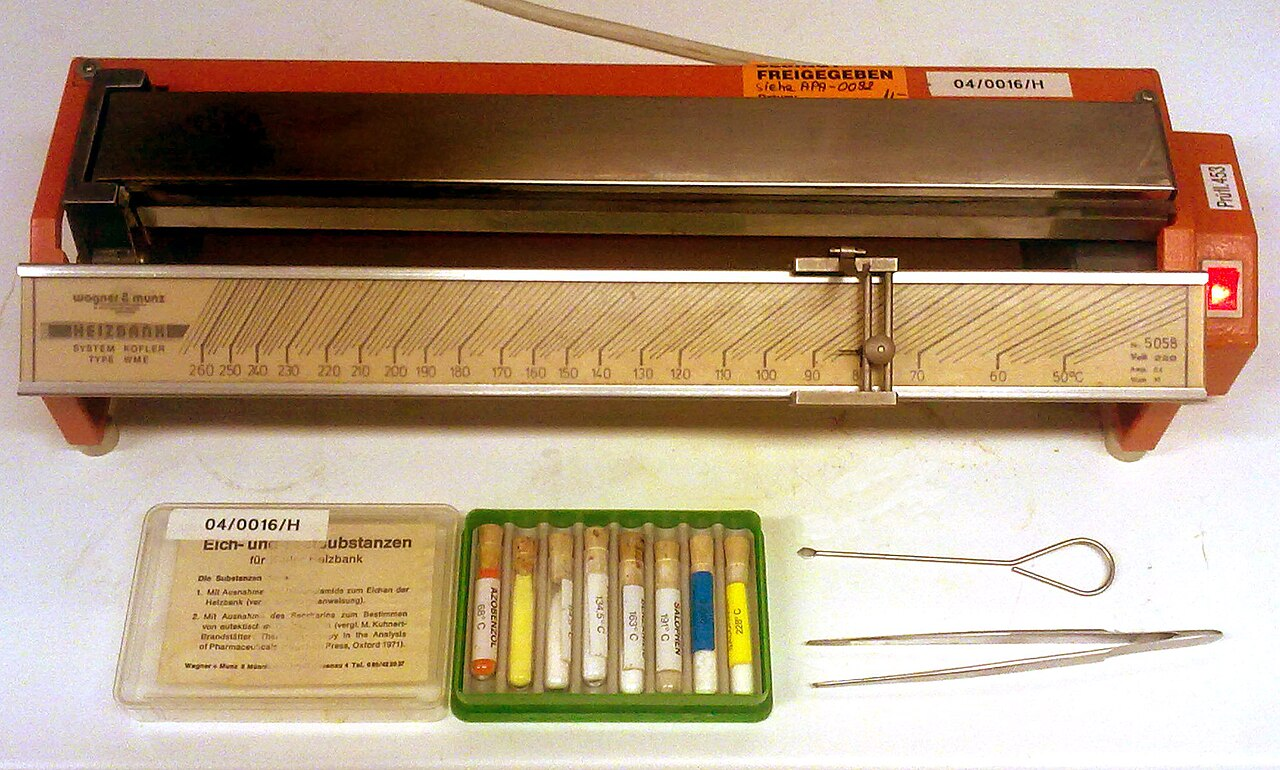
\includegraphics[width=0.62\linewidth]{images/book2/kofler-bench.jpg}

{\small Um banco aquecido (banco de Kofler): uma tira metálica aquecida em
uma das extremidades, com um gradiente de temperatura ao longo dela; o
sólido, espalhado sobre a tira, funde além de uma linha nítida, lida na
escala com o cursor. A caixa guarda substâncias de referência de ponto de
fusão conhecido, usadas para calibrá-lo. Foto: HBR, CC BY-SA 3.0,
Wikimedia Commons.}
\end{omfigure}

\begin{method}[Medir um ponto de fusão em um banco aquecido]\label{met:b1:lab-techniques-1:melting-point}
\begin{enumerate}
  \item Ligue o banco com bastante antecedência: o gradiente leva tempo
        para se estabilizar.
  \item Calibre-o com uma substância de referência pura que funda perto
        do valor esperado, espalhada sobre a tira; ajuste o cursor para que
        a escala indique seu ponto de fusão na linha.
  \item Espalhe alguns \omterm{def:b1:crystals-metals:crystal}{cristais} da amostra seca da extremidade fria para
        a quente; empurre-os para a frente e para trás com a espátula e
        ponha o cursor no limite além do qual o sólido funde de imediato.
  \item Leia, repita, limpe a tira; tome a média das leituras e enuncie a
        incerteza (\cref{met:b1:lab-techniques-1:report-result}).
\end{enumerate}
\end{method}

Uma substância cristalina pura funde de modo nítido em seu ponto de
fusão; uma impura começa a fundir mais abaixo e funde ao longo de uma
faixa de temperaturas, porque a impureza abaixa a temperatura em que o
sólido e o líquido coexistem (a razão, o potencial químico de um solvente
abaixado por um soluto, está no volume do 2.º~ano). Um ponto de fusão
bem abaixo do valor tabelado, ou uma faixa de fusão larga, revela
portanto impurezas; um valor compatível com o tabelado, no sentido do
\omterm{def:b1:lab-techniques-1:z-score}{desvio normalizado}, apoia a pureza sem prová-la.

\begin{inthelab}[Calibrar o banco]
As referências são escolhidas de modo a enquadrar o valor esperado. A
acetanilida, que funde a \qty{114.3}{\celsius}, e o ácido benzoico, a
\qty{122.4}{\celsius}, são padrões clássicos para produtos que fundem entre
\qty{110}{\celsius} e \qty{130}{\celsius}; para a aspirina, um padrão perto
de \qty{135}{\celsius} é melhor ainda. A própria aspirina se decompõe ao
fundir, de modo que seu ponto de fusão observado depende da velocidade de
aquecimento: as tabelas dão \qty{135}{\celsius} para aquecimento rápido,
que é o que um banco faz.
% ledger: mp:acetanilide, mp:benzoic, mp:aspirin
\end{inthelab}

Um líquido é identificado, e sua pureza verificada, por seu \emph{índice
de refração} $n_D$, a razão entre a velocidade da luz no vácuo e sua
velocidade no líquido, medido com a raia D amarela do sódio a uma
temperatura indicada (em geral \qty{20}{\celsius}), com quatro casas
decimais. A água tem $n_D = 1.333$, o etanol 1.3611 e o ciclo-hexano
1.4266 a \qty{20}{\celsius}. O índice diminui ligeiramente quando a
temperatura sobe, de modo que o instrumento é termostatizado.
% ledger: nD:water, nD:ethanol, nD:cyclohexane

\begin{omfigure}
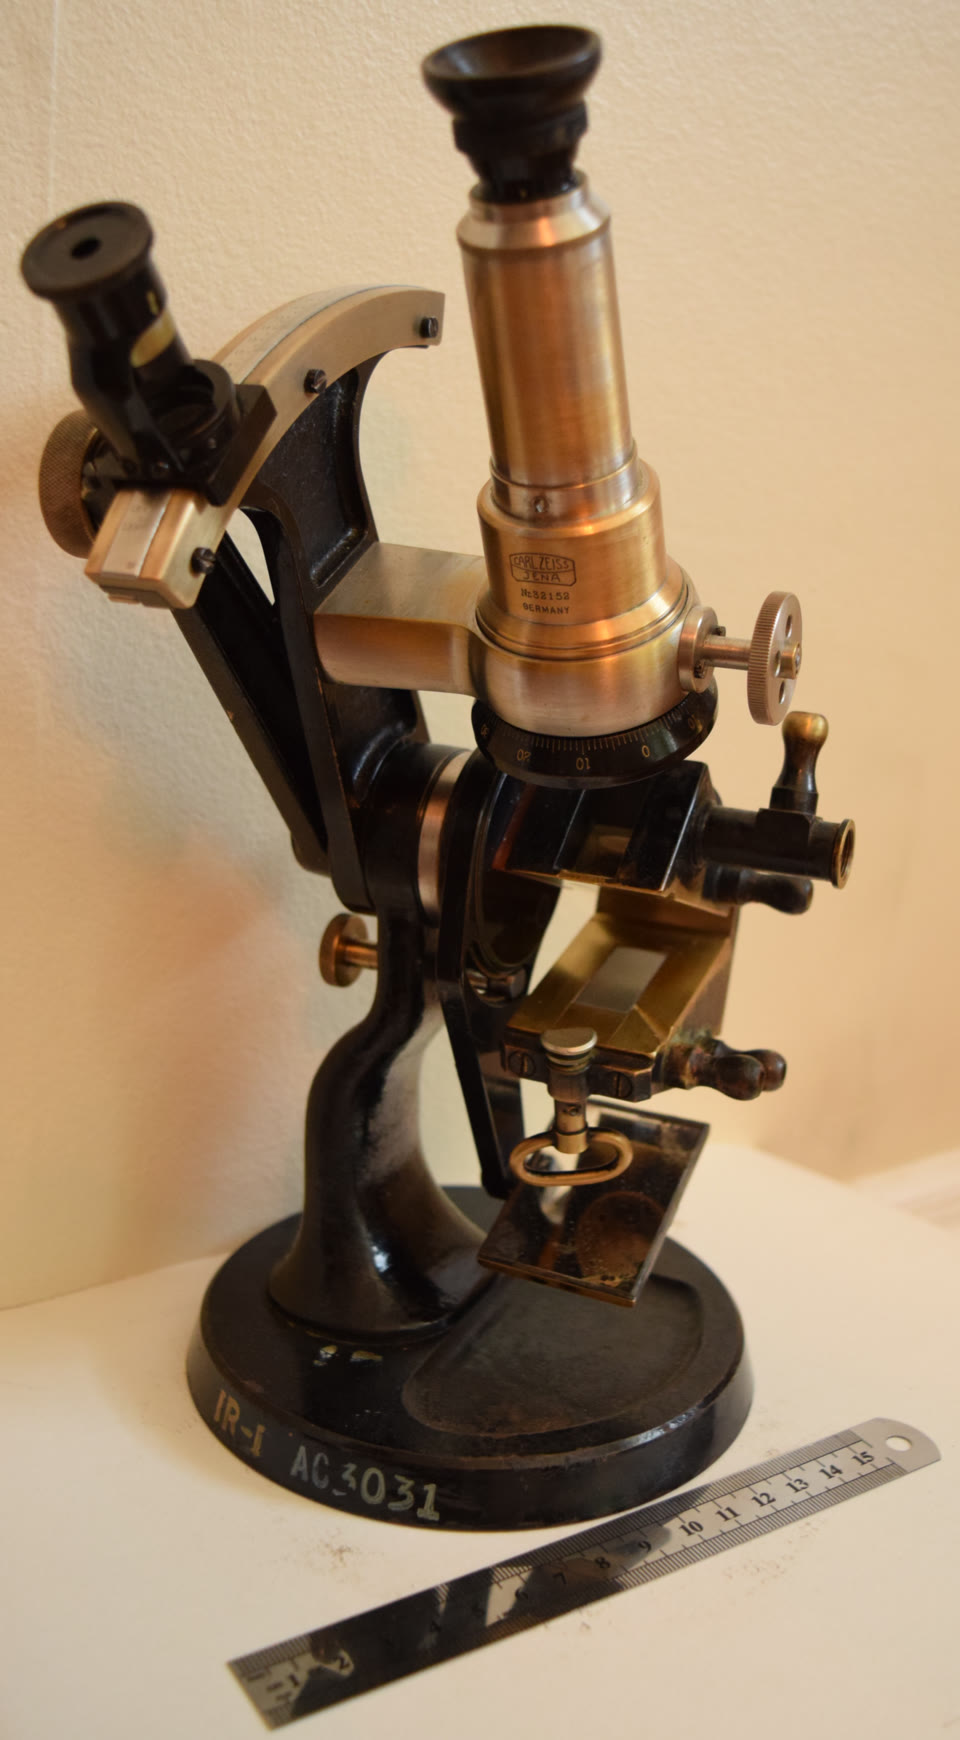
\includegraphics[height=6cm]{images/book2/abbe-refractometer.jpg}

{\small Um refratômetro de Abbe: uma gota de líquido é espalhada entre dois
prismas; a ocular mostra um campo metade claro e metade escuro, e a
fronteira, posta sobre a cruz do retículo, dá o índice de refração na
escala. Foto: Foreade, CC BY-SA 4.0, Wikimedia Commons.}
\end{omfigure}

\section{Exercícios}

\begin{exercise}[$\star$]\label{exo:b1:lab-techniques-1:1}
Um frasco de propanona traz os pictogramas GHS02 e GHS07 e as frases
H225, H319 e H336. Que \omterm{def:b1:lab-techniques-1:ghs}{palavra de advertência} ele traz? Quais frases
descrevem um \omterm{def:b1:lab-techniques-1:hazard}{perigo} físico, quais um \omterm{def:b1:lab-techniques-1:hazard}{perigo} para a saúde? Cite duas
precauções que elas exigem.
\end{exercise}

\begin{exercise}[$\star$]\label{exo:b1:lab-techniques-1:2}
\omterm{def:b1:lab-techniques-1:hazard}{Perigo} ou \omterm{def:b1:lab-techniques-1:hazard}{risco}? (a) O ácido sulfúrico concentrado provoca queimaduras
graves. (b) Pesar \qty{50}{mg} de um pó tóxico em capela, com luvas, expõe
pouco o operador. (c) O sódio libera hidrogênio com a água. (d) O mesmo
solvente é mais perigoso usado quente em um béquer aberto do que frio em
um frasco fechado.
\end{exercise}

\begin{exercise}[$\star$]\label{exo:b1:lab-techniques-1:3}
Em uma placa de CCD, a frente do eluente está a \qty{6.0}{cm} acima da
linha de base; a amostra dá manchas a \qty{2.1}{cm} e \qty{4.2}{cm}.
Calcule seus $R_f$. Uma referência depositada na mesma placa sobe até
\qty{4.2}{cm}: o que se pode e o que não se pode concluir?
\end{exercise}

\begin{exercise}[$\star$]\label{exo:b1:lab-techniques-1:4}
Uma bureta graduada a cada \qty{0.1}{mL} é lida a meia divisão. Calcule a
\omterm{def:b1:lab-techniques-1:uncertainty}{incerteza-padrão} de uma leitura, depois a de um volume fornecido, a
diferença de duas leituras.
\end{exercise}

\begin{exercise}[$\star\star$]\label{exo:b1:lab-techniques-1:5}
Cinco pesagens da mesma amostra dão \qty{0.2512}{g}, \qty{0.2508}{g},
\qty{0.2515}{g}, \qty{0.2510}{g} e \qty{0.2505}{g}. Calcule a média, o
desvio-padrão experimental, a \omterm{def:b1:lab-techniques-1:uncertainty}{incerteza-padrão} da média, e expresse o
resultado com $k = 2$.
\end{exercise}

\begin{exercise}[$\star\star$]\label{exo:b1:lab-techniques-1:6}
Um soluto com \omterm{def:b1:lab-techniques-1:partition-coefficient}{coeficiente de partição} $K = 3$ entre um solvente orgânico e
a água é extraído de \qty{50}{mL} de água com \qty{30}{mL} de solvente no
total. Calcule a fração extraída em uma porção, em duas porções de
\qty{15}{mL} e em três de \qty{10}{mL}.
\end{exercise}

\begin{exercise}[$\star\star$]\label{exo:b1:lab-techniques-1:7}
Uma \omterm{def:b1:titration-methods:titration}{titulação} dá uma concentração de \qty{0.1012}{mol/L} com \omterm{def:b1:lab-techniques-1:uncertainty}{incerteza-padrão}
\qty{0.0006}{mol/L}; a solução foi preparada a \qty{0.1000}{mol/L} com
\omterm{def:b1:lab-techniques-1:uncertainty}{incerteza-padrão} \qty{0.0002}{mol/L}. Os dois valores são compatíveis? E
se a incerteza da \omterm{def:b1:titration-methods:titration}{titulação} tivesse sido de
\qty{0.0004}{mol/L}?
\end{exercise}

\begin{exercise}[$\star\star$]\label{exo:b1:lab-techniques-1:8}
As \omterm{def:b1:precipitation:solubility}{solubilidades} (valores ilustrativos, em \unit{g} por \qty{100}{mL}) de
um sólido em três solventes são: solvente P, 1.5 a frio e 2.0 em
ebulição; solvente Q, 0.3 a frio e 12 em ebulição; solvente R, 9 a frio e
25 em ebulição. Que solvente convém a uma \omterm{def:b1:lab-techniques-1:recrystallisation}{recristalização}, e por que não
os outros dois? Com o solvente certo, qual é a maior fração de
\qty{5.0}{g} do sólido que pode ser recuperada, se for usado o mínimo de
solvente em ebulição e a mistura for resfriada?
\end{exercise}

\begin{exercise}[$\star\star$]\label{exo:b1:lab-techniques-1:9}
Um líquido incolor, termostatizado a \qty{20}{\celsius}, tem
$n_D = 1.3612$. Ele pode ser água, etanol ou ciclo-hexano? Por que a
temperatura é indicada? O que sugeriria um valor de 1.350?
\end{exercise}

\begin{exercise}[$\star\star\star$]\label{exo:b1:lab-techniques-1:10}
Com os dados do \cref{exo:b1:lab-techniques-1:6}, mostre que, por mais
finamente que os \qty{30}{mL} de solvente sejam divididos, no máximo uma
fração $1 - \mathrm{e}^{-KV/V_a}$ do soluto pode ser extraída, e
calcule-a. Quantas porções atingem \qty{99}{\percent} desse limite?
\end{exercise}

\begin{exercise}[$\star\star\star$]\label{exo:b1:lab-techniques-1:11}
Uma grandeza é conhecida por estar entre $x_0 - a$ e $x_0 + a$, sendo os
valores perto de $x_0$ mais prováveis: sua densidade é triangular, $(a - |x - x_0|)/a^2$.
Verifique que ela é normalizada e mostre que sua \omterm{def:b1:lab-techniques-1:uncertainty}{incerteza-padrão} é
$a/\sqrt6$. Compare com o caso retangular.
\end{exercise}

\begin{exercise}[$\star\star\star$]\label{exo:b1:lab-techniques-1:12}
Uma solução-padrão é preparada dissolvendo a amostra do
\cref{exo:b1:lab-techniques-1:5} (massa molar \qty{204.2}{g/mol}, de
incerteza desprezível) em um balão volumétrico de \qty{100.00}{mL} cujo
volume tem uma \omterm{def:b1:lab-techniques-1:uncertainty}{incerteza-padrão} de \qty{0.06}{mL}. Calcule a
concentração e suas \omterm{def:b1:lab-techniques-1:uncertainty}{incertezas relativa} e expandida. Que fonte
domina?
\end{exercise}

\section{Problema: purificar a aspirina}

\begin{problem}[{Problema de fim de semana --- os perigos de uma síntese,
a recristalização da aspirina bruta e seu rendimento, um ponto de fusão
com suas incertezas dos tipos A e B, e o desvio normalizado em relação ao
valor tabelado}]
\label{pb:b1:lab-techniques-1:1}
Uma estudante prepara aspirina aquecendo \qty{2.00}{g} de ácido
salicílico com excesso de anidrido etanoico, e depois recristaliza o
produto bruto. Massas molares (\unit{g/mol}): ácido salicílico \ce{C7H6O3} 138.0, aspirina
\ce{C9H8O4} 180.0, anidrido etanoico \ce{C4H6O3} 102.0. Rótulos:
ácido salicílico GHS05, GHS07, H302, H318; anidrido etanoico GHS02,
GHS05, GHS06, GHS07, H226, H302, H314, H332; aspirina GHS07, H302.
\omterm{def:b1:precipitation:solubility}{Solubilidade} da aspirina em água: \qty{3.3}{g/L} a \qty{25}{\celsius}.
Ponto de fusão tabelado da aspirina (aquecimento rápido): \qty{135}{\celsius}.
% ledger: ghs:salicylic, ghs:acetic-anhydride, ghs:aspirin, sol:aspirin-25,
% mp:aspirin, hstat:H318, hstat:H226, hstat:H314, hstat:H302

\medskip
\noindent\textbf{Parte I --- Os \omterm{def:b1:lab-techniques-1:hazard}{perigos}.}
\begin{enumerate}
  \item O que significa cada pictograma do rótulo do anidrido etanoico?
  \item Que \omterm{def:b1:lab-techniques-1:ghs}{palavra de advertência} traz o rótulo do ácido salicílico? E o
        da aspirina?
  \item O anidrido etanoico tem os \omterm{def:b1:lab-techniques-1:hazard}{perigos} mais graves. Explique como o
        \omterm{def:b1:lab-techniques-1:hazard}{risco} de manipular \qty{5}{mL} dele pode, ainda assim, ser tornado pequeno.
  \item Quais frases do anidrido exigem óculos e luvas, e quais exigem a
        capela e a ausência de chamas?
  \item O que se faz de imediato se uma gota de anidrido atingir um olho?
  \item O filtrado da \omterm{def:b1:lab-techniques-1:recrystallisation}{recristalização} contém ácido etanoico e um pouco de
        etanol em água. Para onde ele vai?
\end{enumerate}

\noindent\textbf{Parte II --- Síntese e \omterm{def:b1:lab-techniques-1:recrystallisation}{recristalização}.}
\begin{enumerate}[resume]
  \item Escreva a equação da síntese, com o ácido etanoico \ce{C2H4O2}
        como subproduto, e verifique que ela está balanceada.
  \item Calcule a quantidade de matéria de ácido salicílico e a massa
        máxima de aspirina.
  \item O produto bruto seco pesa \qty{2.41}{g}. Por que a
        \omterm{def:b1:lab-techniques-1:recrystallisation}{recristalização} não pode ser dispensada, embora isso seja
        \qty{92}{\percent} do máximo?
  \item A aspirina é recristalizada em um pouco de etanol completado com
        água quente. Por que a \omterm{def:b1:precipitation:solubility}{solubilidade} em água a \qty{25}{\celsius},
        comparada com a \omterm{def:b1:precipitation:solubility}{solubilidade} perto da ebulição, é a propriedade que importa?
  \item Por que o sólido bruto é dissolvido no mínimo de solvente quente?
  \item Por que a solução é resfriada lentamente, e depois em gelo?
  \item \qty{40}{mL} de filtrado a \qty{25}{\celsius} saem do funil, e
        depois \qty{5}{mL} de água de lavagem. Estime a massa de aspirina
        perdida com eles.
  \item O produto puro e seco pesa \qty{1.95}{g}. Calcule o \omterm{def:b1:extent-q-and-k:fractional-extent}{rendimento}.
\end{enumerate}

\noindent\textbf{Parte III --- O ponto de fusão.}
\begin{enumerate}[resume]
  \item Seis leituras no banco, calibrado logo antes, dão 134, 135,
        133, 135, 134 e \qty{136}{\celsius}. Calcule a média.
  \item Calcule o desvio-padrão experimental.
  \item Deduza a \omterm{def:b1:lab-techniques-1:uncertainty}{incerteza-padrão} do tipo A da média.
  \item Cada leitura é feita ao grau mais próximo. Calcule a incerteza de
        leitura do tipo B.
  \item A calibração do banco é garantida a
        $\pm\qty{1}{\celsius}$. Calcule a incerteza do tipo B
        correspondente e depois a \omterm{def:b1:lab-techniques-1:uncertainty}{incerteza-padrão} combinada.
  \item Expresse o ponto de fusão com sua \omterm{def:b1:lab-techniques-1:uncertainty}{incerteza expandida} ($k = 2$).
  \item O produto bruto de um colega funde entre 120 e
        \qty{128}{\celsius}. O que isso indica?
\end{enumerate}

\noindent\textbf{Parte IV --- Comparação com a referência.}
\begin{enumerate}[resume]
  \item O valor tabelado é dado na unidade. Que \omterm{def:b1:lab-techniques-1:uncertainty}{incerteza-padrão} isso
        implica?
  \item Em uma placa de CCD (frente a \qty{6.0}{cm}), o produto bruto mostra
        manchas a \qty{2.3}{cm} e \qty{3.3}{cm}, o ácido salicílico uma
        mancha a \qty{2.3}{cm}, o produto recristalizado uma mancha a
        \qty{3.3}{cm}. Calcule os valores de $R_f$ e conclua.
  \item Por que o ponto de fusão da aspirina depende da velocidade de
        aquecimento?
  \item Calcule o \omterm{def:b1:lab-techniques-1:z-score}{desvio normalizado} $z$ entre os pontos de fusão medido e
        tabelado, e diga se eles são compatíveis.
\end{enumerate}
\end{problem}
